\section{Model assesment \& selection}

\textcolor{gray}{The following considerations hold for all supervised learning methods, for simplicity we'll focus on classification methods.}
\vspace{0.2cm}
Once we've trained a classifier we're interested in evaluating the model on new observations drawn from the same population.

We have some data model $\mathcal{D} = \{(x_i, y_i)\}_{i=1}^n$ on which we train a model $\hat{f}_{\mathcal{D}}(x)$.\\
To evaluate our model we need to known the error it will make on future data, in other words we want the \textbf{expected misclassification error}:
$$
Err = \expect_{(X,Y)}[L(\ Y,\ \hat{f}_{\mathcal{D}}(X)\ )]
$$
where $L$ is a simple \textbf{loss function} returning 0 if the prediction is correct 1 otherwise.\\

To do this we take an independent set to \textbf{test our model} $\mathcal{D}_{test} = \{(x_i, y_i)\}_{i=1}^m$ and on this new dataset we compute the misclassification error:
$$
\widehat{Err}_{test} =  \frac{1}{m}\sum_{i=1}^{m} L(y_i, \hat{f}_{\mathcal{D}}(x_i))
$$
\begin{figure}[h]
    \centering
    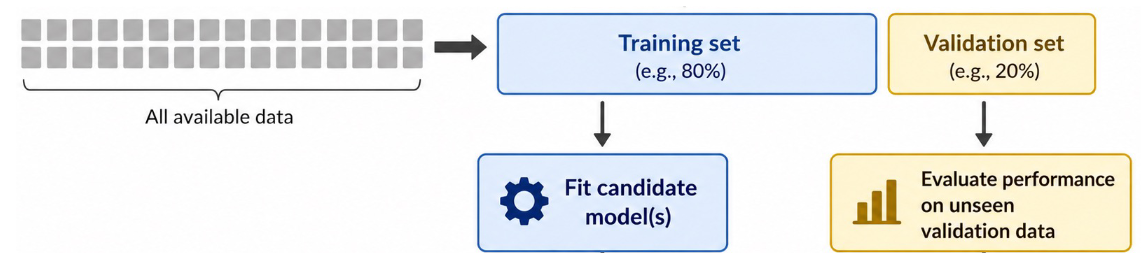
\includegraphics[width=0.5\linewidth]{img//model_selection/train_test_split.png}
\end{figure}\hfill\\
Thanks to the fact the observations in the dataset are different datapoints, this metric si better in evaluating our model with respect to $\widehat{Err}_{train}$: training erro is typically optimistically biased, especially with very flexible models.
\begin{figure}[h]
    \centering
    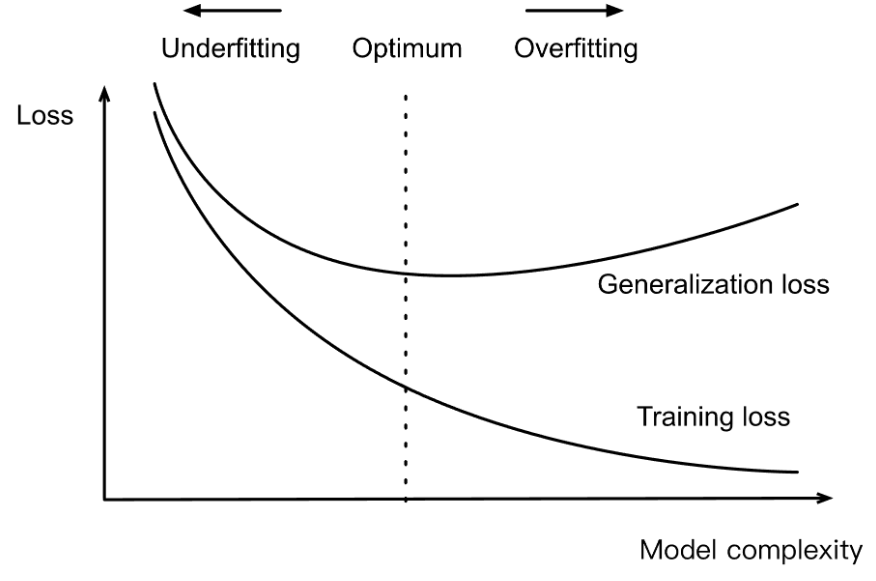
\includegraphics[width=0.4\linewidth]{img//model_selection/train_test_error_comparison.png}
\end{figure}

\vspace{0.2cm}
However this approach is not prefect: if we get unlucky the result of the validation set might be highly biased by the division, and we are "wasting" some data that could potentially be used for training a better model.

\newpage
\subsection{K-fold Cross-Validation (CV)}
The idea is to split the whole data in \textbf{k-folds} $\mathcal{D}= \mathcal{D}_1,\mathcal{D}_2\ ...\mathcal{D}_K $ and $\forall$  fold $k$ train the model on the remaining folds and test it on $\mathcal{D}_k$.At the end we validate the model on the \textbf{cross-validation estimate} \textcolor{gray}{(just the average of all fold's misprediction error)}:
$$
CV_K = \frac{1}{K}\sum_{k=1}^{K} \frac{1}{|D_k|}\sum_{i \in D_k} L(y_i, \hat{f}^{(-k)}(x_i))
$$
\begin{figure}[h]
    \centering
    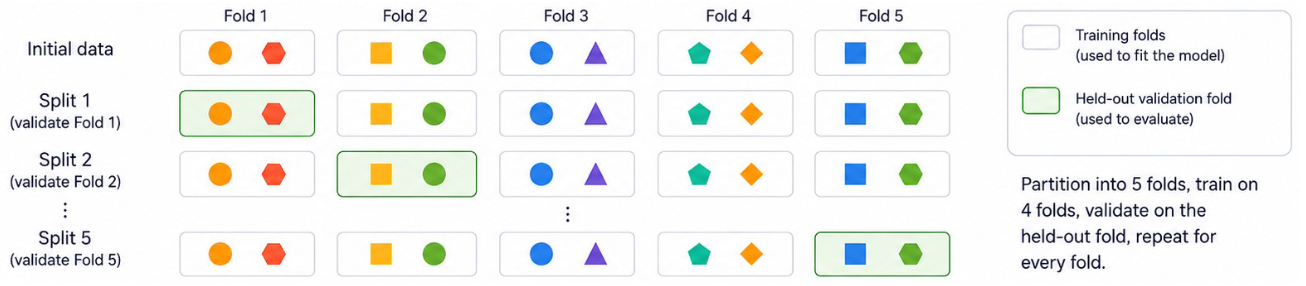
\includegraphics[width=0.8\linewidth]{img//model_selection/cross_validation.png}
\end{figure}

\vspace{0.2cm}
\textbf{Note}: cross-validation can be used both for \textit{model assessment} (how well my model generalize the data, evaluating the model on the CV) and \textit{model selection} (which model shoudl we choose, choosing the model that minimizes the CV error)
\vspace{0.2cm}

The cross-validation technique allows us to visualize the \textbf{overfitting} problem: the more the model overfits the more the CV error increases w.r.t. training error.
\begin{figure}[h]
    \centering
    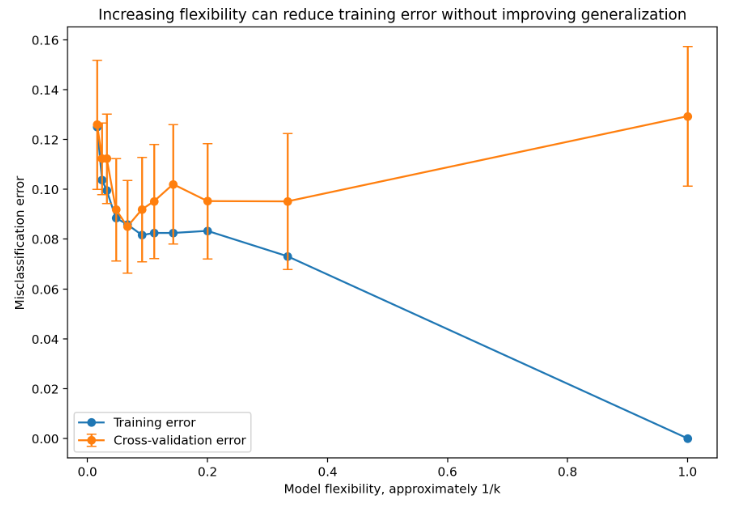
\includegraphics[width=0.5\linewidth]{img//model_selection/overfitting_visualized.png}
\end{figure}
\vspace{0.2cm}
Another thing worth of beding visualized is the mean and the std deviation of the error across different folds, in order to get an idea of the CV variability (however these are not CIs since the sets are not indepenent).
\begin{figure}[h]
    \centering
    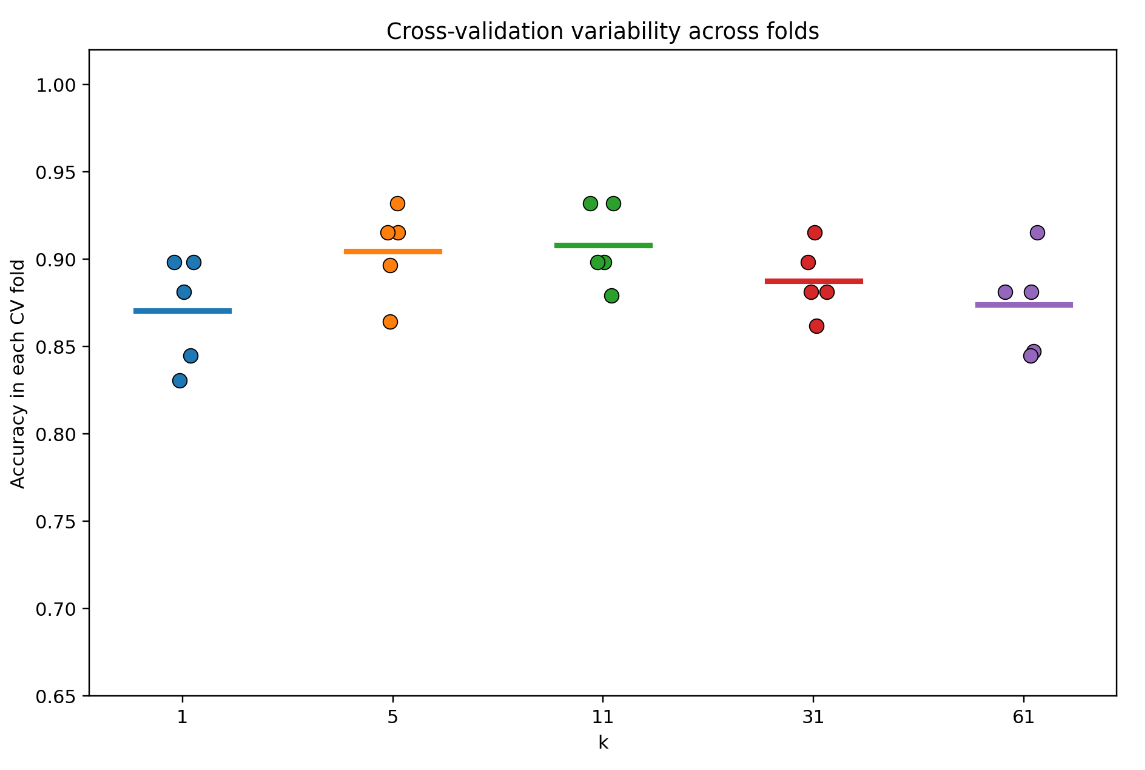
\includegraphics[width=0.5\linewidth]{img//model_selection/cv_variability.png}
\end{figure}

\subsection{Bootstrapping}
CV helps understanding the goodness of our model in generalizing data and might help in choosing the hyperparameters. However usually we'd like to understand \textit{how variable/stable is our result}.
\vspace{0.2cm}
The idea is to use our dataset as population and simulate a new "dataset" by sampling from it \textcolor{gray}{(this method is used also outside the supervised learning framework)}.
\begin{enumerate}
    \item we sample with replacement $n$ observations from \dataset: $\mathcal{D}^{*b}=\{z_1^{*b}...z_n^{*b}\}$:= \textbf{boostrap sample} for $b=1...B$ 
    \item compute some statistic (any kind) on the boostrap sample $\hat{\theta}^{*b}=s(\mathcal{D}^{*b})$
    \item we use the distribution of the statistics $\hat{\theta}^{*1}...\hat{\theta}^{*B}$ to estimate that uncertanty, like uncertanty intervals \arrow for example we can build percentile intervals $[q_{0.025}(\hat{\theta}^*),q_{0.975}(\hat{\theta}^*)]$
\end{enumerate}

In supervised learning we use the boostraping to fit a model $\hat{f}^{*b}()$ on each boostrap sample $\mathcal{D}^{*b}$ (each data sampled is a pair $(x_i,y_i)$, allowing us to verify several quantities across different models:\\
\begin{itemize}
    \item we can check the \textbf{variability of the model parameters} of the regression coefficients $\hat{\beta}_j^{*1}...\hat{\beta}_j^{*B}$
    \item we can check for the \textbf{variability of the prediction} $\hat{f}^{*1}(x_0)...\hat{f}^{*B}(x_0)$ on a fixed point $x_0$
    \item we can check the \textbf{variability of the model performance}
\end{itemize}
For example in \textit{KNN} we can use to bootstrap both to check the stability of the parameter $k$, to check the stability of the AUC or even to check the stability of the predictors.\\
\vspace{0.3cm}
The replacement in the bootstraping is essetial, but causes some observations to never been selected. Given $n$ observations, we have that the probabilityof each observation of not bein selected is:
$$
\left(1-\cfrac{1}{n}\right)^n\approx e^{-1}\approx 0.368
$$
the set of observations left-out is called the \textbf{out-of-bag} observations.
\begin{figure}[h]
    \centering
    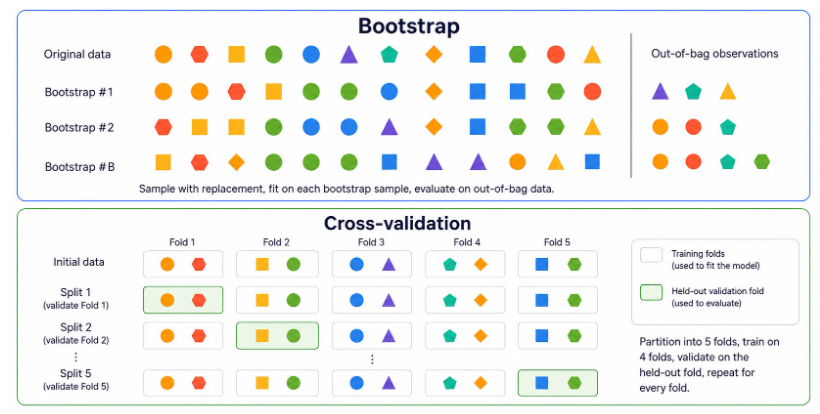
\includegraphics[width=0.7\linewidth]{img//model_selection/boostrap_example.png}
\end{figure}